\documentclass[sigconf]{acmart}

\usepackage[utf8]{inputenc}
\usepackage{listingsutf8}
\usepackage{balance}
\usepackage{booktabs}
\usepackage{multirow}
\usepackage{tabularx}
\usepackage{adjustbox}
\usepackage{makecell}
\usepackage{microtype}
\usepackage{xurl}
\usepackage{seqsplit}
% --- Padronizacao visual (tabelas e quebras de linha) ---
\setlength{\tabcolsep}{4pt}
\renewcommand{\arraystretch}{1.1}
\setlength{\emergencystretch}{2em}
\newcommand{\tcode}[1]{\texttt{\seqsplit{#1}}}

\setcopyright{none}
\settopmatter{printacmref=false}
\renewcommand\footnotetextcopyrightpermission[1]{}


\title{Lacunas na Fusão de Operadores em Sistemas de Deep Learning: O \textit{Trade-off} entre Compilação e Execução de Operações Não Fundidas}

\newcommand{\statci}[4]{\num{#1}\,$\pm$\,\num{#2}\,[\num{#3},\,\num{#4}]}
\newcommand{\best}[1]{\textcolor{blue}{#1}}
\newcommand{\worst}[1]{\textcolor{red}{#1}}

\renewcommand\abstractname{ABSTRACT}
\renewcommand\keywordsname{KEYWORDS}
\renewcommand\refname{REFERENCES}

\author[G. Guimar\~{a}es]{Gabriel Guimar\~{a}es dos Santos Ricardo}
\affiliation{%
  \institution{UFMG}
  \city{Belo Horizonte}
  \country{Brazil}}
\email{gabriel.guimaraes@dcc.ufmg.br}

\author[N. Santos]{Natanael dos Santos Junior}
\affiliation{%
  \institution{UFMG}
  \city{Belo Horizonte}
  \country{Brazil}}
\email{natanaeljunior@dcc.ufmg.br}

\author[F. Figueiredo]{Flavio Figueiredo}
\affiliation{%
  \institution{UFMG}
  \city{Belo Horizonte}
  \country{Brazil}}
\email{flaviovdf@dcc.ufmg.br}

\author[F. Pereira]{Fernando Magno Quint\~{a}o Pereira}
\affiliation{%
  \institution{UFMG}
  \city{Belo Horizonte}
  \country{Brazil}}
\email{fernando@dcc.ufmg.br}
\date{September 2025}\begin{document}

\begin{abstract}
Operator fusion trades compilation time for execution efficiency, but this cost is often hidden. In modern compilers such as PyTorch 2 \(TorchInductor\) and XLA, heuristics and constraint rules prevent the fusion of common kernels like BatchNorm+ReLU and BatchNorm → Conv, which, if fused, can affect both compilation and execution times. In this paper, we algebraically formalize the trade-off between compilation-time and execution-time gains during Operator Fusion passes in modern machine learning compilers. We also prove that, with respect to time-to-first-batch, PyTorch 2 performs fusion passes in a suboptimal order, and we propose an alternative optimization sequence. Finally, we provide a real-world benchmark and a tool to indicate the best backend according to the usage regime.
\end{abstract}

\maketitle
\noindent\large{\textbf{KEYWORDS}} \\ Large-Language Model, Hardware Performance, Performance Prediction


\section{Introduction}
A técnica de \emph{fusão de operadores} tem raízes diretas em otimizações clássicas de compiladores, como a fusão de \emph{loops}, historicamente empregada para aumentar paralelismo e melhorar a localidade de dados \cite{wolf1991wolf}. Em compiladores modernos para Aprendizado de Máquina, particularmente em GPUs, essa técnica assume um papel central: ao combinar múltiplas operações em um único \emph{kernel}, reduz-se o tráfego de memória, evitam-se tensores intermediários e diminui-se o número de disparos dinâmicos durante a execução \cite{chen2018tvm,liu2021dnnfusion}. Sistemas como XLA, TVM, TensorRT e o backend TorchInductor adotam fusão agressiva para amortizar custos de comunicação CPU–GPU e consolidar sequências de operadores em \emph{kernels} maiores e mais eficientes \cite{xla2017leary,chen2018tvm,pytorch2022}.

A fusão é realizada sobre o grafo de fluxo de controle (CFG) do programa. Entretanto, decidir \emph{o que} e \emph{como} fundir em grafos modernos é desafiador: planos ótimos de fusão são, em geral, problemas NP-difíceis \cite{darte1999,10.5555/645671.665526}. Por isso, compiladores adotam heurísticas que buscam equilibrar \textbf{tempo de compilação} e \textbf{tempo de execução}. Esse equilíbrio é especialmente importante em cargas dinâmicas (com \emph{shapes} variáveis) e em cenários com poucas repetições, nos quais o custo até a primeira execução domina o desempenho percebido.

Apesar desse impacto, a literatura usualmente privilegia métricas de latência e ignora o tempo de compilação. Falta um protocolo que torne explícita a relação entre \emph{compilar mais para executar menos} e \emph{compilar rápido com menos fusões}, permitindo orientar a escolha prática de \emph{backend}. Compiladores como XLA \cite{snider2023xla}, TVM \cite{chen2018tvm} e TorchInductor (PyTorch~2) \cite{pytorch2022} adotam estratégias distintas — regras estáticas, exploração ou auto-\emph{tuning}, e \emph{codegen} local — o que resulta em perfis muito diferentes de tempo de compilação e de execução.

Foi avaliado o \emph{trade-off} entre esses dois tempos nos compiladores TVM, XLA e TorchInductor sob um protocolo comum. Para um número de execuções \(n\), estimamos qual \emph{backend} minimiza o parâmetro \(T_b(n)=a_b n + b_b\), apresentado na Seção~4.3. Foi investigado também as heurísticas de fusão utilizadas pelos compiladores e foi proposto uma nova ordem de execução que reduz simultaneamente o tempo de compilação e o de execução em modelos reais.

\textbf{Como Contribuições}
\begin{itemize}
    \item Formulação algébrica do trade-off entre tempo de compilação e execução de modelos de ML (\textit{Machine Learning}) em respeito às heurísticas de fusão de \textit{kernels};
    \item Análise e benchmarking dos modelos XLA, PyTorch e TVM em termos do nosso arcabouço algébrico;
    \item Análise de artefatos (TVMScript, HLO, Triton) para quantificar e analisar a granularidade de fusão por \emph{backend}, mapeando padrões por arquitetura (ResNet-18/50, BERT e GPT-2) e seus impactos em latência;
    \item Proposta de uma nova ordem de otimização para o PyTorch durante a Fusão;
\end{itemize}

\section{Methodology}

Comparamos \textit{TVM} \cite{chen2018tvm}, \textit{XLA} \cite{snider2023xla} e \textit{TorchInductor} (PyTorch~2) \cite{pytorch2022} em ambiente controlado, medindo \textbf{tempo de compilação}, \textbf{latência média por execução} e \textbf{granularidade de fusão}.

\subsection{Ambiente Experimental}

Todos os experimentos foram executados no mesmo sistema computacional. O ambiente base consiste em um sistema operacional Fedora~41, utilizando o kernel~6.16.12, com CPU AMD Ryzen~5~4600G e 15{,}4~GiB de memória RAM. A GPU utilizada foi uma NVIDIA RTX~3050 com 8~GB de memória, operando com o driver versão~580.95.05. A pilha CUDA foi composta pelo driver CUDA~13.0 e pelo compilador \textit{nvcc} versão~12.6 (V12.6.77).

\paragraph{Configuração por framework.}
Para os experimentos com \textbf{TVM}, utilizou-se o Python~3.11.13, cuDNN versão~9.1 (via PyTorch), TVM~0.22.dev0 (commit~3b60f1c), LLVM~20.1.8 e CUDA~12.6 integrado ao backend do TVM.

No caso do \textbf{XLA/TorchInductor}, os experimentos foram conduzidos com Python~3.10.18. O backend XLA utilizou JAX/jaxlib~0.6.2, com PJRT (\tcode{jax-cuda12-pjrt}~0.6.2) e cuDNN~9.10.2.21 instalado via \textit{pip}. Para o TorchInductor, utilizou-se PyTorch~2.5.1+cu121, com execução no dispositivo \tcode{cuda:0}.


Utilizamos o mesmo hardware/OS e \emph{stack} de software por \emph{backend}, conforme a Tabela ~\ref{tab:env-condensado}. Condições padronizadas: \tcode{TF32} ativado, layout \textit{channels\_last}, \tcode{cudnn.benchmark=True}, todos os modelos em \tcode{eval()}, \emph{warmup} e separação explícita entre compilação e execução. Utilizamos um ambiente isolado para o \textbf{TVM} na versão \tcode{0.22.dev0}.

\subsection{Modelos e entradas}
Avaliamos \textbf{ResNet-18/50}, \textbf{BERT} e \textbf{GPT-2}. Entradas para Resnets (CNNs): \tcode{(1,3,224,224)}, \tcode{(16,3,224,224)}, \tcode{(64,3,224,224)}, \tcode{(1,3,512,512)}, \tcode{(1,3,1024,1024)}. Entradas para Transformers: pares \tcode{(batch, seq\_len)} em \tcode{(1,64)}, \tcode{(1,128)}, \tcode{(8,128)}.

Os modelos \textbf{ResNet-18/50}, \textbf{BERT} e \textbf{GPT-2} foram escolhidos por representarem padrões arquiteturais distintos e complementares. As ResNets caracterizam arquiteturas convolucionais clássicas, com cadeias recorrentes do tipo \textit{Conv--BatchNorm--ReLU}, que são casos canônicos para análise de fusão de operadores em CNNs. 

O BERT representa arquiteturas \textit{Transformer} baseadas em codificadores, dominadas por multiplicações de matrizes, projeções lineares, normalizações e ativações, permitindo avaliar estratégias de fusão em grafos centrados em atenção. 

O GPT-2, por sua vez, exemplifica modelos \textit{decoder-only} autoregressivos, com fluxo computacional mais linear e repetitivo, típico de modelos generativos, nos quais a granularidade das fusões impacta diretamente a latência de inferência. 

Em conjunto, esses modelos permitem analisar o comportamento das heurísticas de fusão em diferentes regimes computacionais e arquiteturais.

\subsection{Pipeline experimental}
\label{sec:pipeline}
O fluxo do benchmark adota quatro etapas sequenciais, padronizadas para todos os modelos e backends (TVM, XLA e TorchInductor):

\paragraph{(1) Compilação.}
Para cada par \textit{(modelo, entrada)}, é registrado o tempo de compilação
%o grafo é enviado em modo de compilação, registrando-se o tempo de compilação 
(\tcode{compile\_ms}) em um processo isolado e versões fixas de drivers e bibliotecas com foco principal no custo de geração de código.

\paragraph{(2) Warmup e execução + captura do grafo.}
A execução ocorre em duas fases: (i) fase de \textit{warmup}, focada em construir caches e realizar \textit{autotuning}; e (ii) fase das \textit{execuções válidas} e cronometradas. Durante (ii), o benchmark exporta os CFG's das representações intermediárias (IR's) dos backends analisados [HLO (XLA), TVMScript e TIR (TVM),  IR e Triton (TorchInductor)]. Também coletamos metadados dos \textit{kernels} quando disponíveis. 

\paragraph{(3) Análise da quantidade e qualidade dos \textit{kernels}.}
A partir das IRs capturadas, realizamos uma análise estrutural dos \textit{kernels} gerados por cada backend. Essa etapa inclui a quantificação do número total de \textit{kernels}, a distinção entre \textit{kernels} internos e chamadas a bibliotecas externas, bem como a caracterização qualitativa das fusões realizadas. Essa análise permite avaliar a granularidade das fusões e o grau de delegação a bibliotecas otimizadas, fornecendo contexto estrutural para a interpretação dos resultados de desempenho.


\paragraph{(4) Medições e modelo algébrico.}
As métricas coletadas incluem: \textit{Tempo até o primeiro batch} (\tcode{ttfb\_ms}), \textit{latência média por execução} $a$ e \textit{desvio-padrão} nas 50 execuções válidas (\tcode{exec\_ms\_mean}, \tcode{exec\_ms\_std}). Para \textbf{XLA/TVM}, separa-se \textbf{explicitamente} o tempo de compilação da primeira chamada compilada $b$. Para \textbf{TorchInductor}, o tempo de compilação é estimado por
\[
\mathrm{compile\_time}=\mathrm{first\_call\_ms}-\mathrm{time\_per\_run\_ms},
\]
em que \textit{first\_call\_ms} agrega compilação+execução e \textit{time\_per\_run\_ms} é a média das execuções subsequentes. 

\textbf{\textit{Modelo algébrico.}}
Nós propomos um modelo algébrico para o cálculo do custo da compilação e execução em lotes nos três backends analisados dado por:
\[
T_b(n) = a_b\,n + b_b,
\]
em que $b_b$ é o custo fixo de compilação e sobrecarga inicial e $a_b$ a latência média, permitindo inferir o ponto de inflexão para diferentes backends em função do número de repetições $n$.

% vamos melhorar essa parte. envoltória inferior?
O modelo \(T_b(n) = a_b n + b_b\), junto da sua \emph{envoltória inferior} --- a curva que, para cada valor de \(n\), seleciona o menor custo entre todos os backends --- ajuda a explicar os pontos de troca observados entre os diferentes \emph{backends}. Assim, as interseções dessas funções indicam a partir de qual tamanho de entrada \(n\) cada backend passa a ser mais vantajoso.

\paragraph{(5) Aplicação de \textit{fold} e comparação de regimes.}
Além do modelos padrões, foi avaliado um cenário alternativo no qual uma transformação de \textit{fold} é aplicada \textbf{antes} da fusão regular de operadores. O \textit{fold} consiste em uma reparametrização algébrica que absorve operações lineares (como \textit{BatchNorm} ou a parte afim da \textit{LayerNorm}) nos parâmetros do operador subsequente, removendo explicitamente essas operações do grafo em modo de inferência.

Diferentemente da fusão de operadores, que combina múltiplas operações em um único \textit{kernel} durante o \textit{codegen}, o \textit{fold} simplifica estruturalmente o grafo antes da geração de código. Como consequência, o \textit{fold} impacta principalmente o custo fixo de compilação, reduzindo a complexidade do \textit{codegen}, enquanto seus efeitos sobre a latência por execução tendem a ser menores ou não determinísticos.

Para as operações com fold, assume-se $T_f(n) = a_f \, n + b_f $ o custo em backends que realizam a operação \textit{fold} antes da fusão de operadores regular. Dessa forma, o ponto de equivalência do número de \textit{batches} $n$ para o qual $\Delta T = T_f(n) - T_b(n) = 0$, sendo $T_b(n)$ o custo no backend compilado sem a operação fold, se dá por:
\begin{align*}
n_{\text{eq}}
  = MAX(0, \frac{b_b - b_f}{a_f - a_b}),
   \qquad \text{desde que } \Delta a \neq 0.
\end{align*}

%[X:] para colocar na apresentação!!! junto com os modelos algébricos. e passar por eles rapidamente durante a apresentação.
% \begin{itemize}
%     \item Se $\Delta b < 0$, então o Fold \textbf{reduz o tempo de compilação}.
%     \item Se $\Delta b > 0$, então o Fold \textbf{aumenta o tempo de compilação} (pior).
%     \item Se $\Delta a < 0$, então o Fold \textbf{reduz o tempo por batch} (execução mais rápida).
%     \item Se $\Delta a > 0$, então o Fold \textbf{aumenta o tempo por batch} (execução mais lenta).
% \end{itemize}

\paragraph{(6) Construção do JSON.}
Para cada \textit{(modelo, entrada, backend)}, incluindo também os modelos com \tcode{fold}, geramos um \tcode{JSON} que consolida o estado do benchmark. Inclui identificação do experimento, métricas de tempo, \textit{kernels} fundidos, e outros metadados. 

%[X: Esse paragrafo abaixo é importante, mas apenas na apresentacao, que vc deve focar na parte da engenharia!!! e do trabalho que foi. mas nao cabe no paper ]

% Todos os arquivos são versionados e nomeados de forma determinística (\textit{timestamp}, \textit{hash} da configuração e \textit{commit} do repositório), de modo que cada resultado possa ser reproduzido e auditado a partir do pacote de artefatos.

\subsection{Execução por compilador e modelo}
Para cada par (\textbf{compilador}, \textbf{modelo}), executamos o pipeline [Seção~\ref{sec:pipeline}]: (i) compilação do grafo, (ii) preparação das entradas, (iii) execução do protocolo escolhido (10 \emph{warmup}'s e $n = 50$), (iv) computamos média, desvio padrão e IC (95\%), e (v) exportamos métricas e artefatos.

\subsection{Script de análise de artefatos (TVMScript, HLO, Triton)}
Implementamos um \textbf{script em Python} que faz o \emph{parsing} textual a árvore do programa e produz um artefato. 

%[X: também cortei isso, mas deve colocar no README.txt do repositorio com link para o paper quando houver]
% produz um relatório estruturado por (\emph{backend}, modelo, forma):
% \begin{itemize}
%     \item \textbf{Contagem de kernels} internos/externos (\emph{únicos} e \emph{totais}).
%     \item \textbf{Listagem de kernels externos} (nomes de \textit{custom-calls}/bibliotecas).
%     \item \textbf{Mapeamento de fusões por kernel interno}:
%     \begin{itemize}
%         \item \textit{TorchInductor}: usa comentários na IR Triton/C++ que enumeram operações fundidas por \emph{kernel} (extração via \tcode{regex}).
%         \item \textit{TVM}: utiliza nomes compostos dos \emph{kernels} (e.g., \tcode{fused\_add\_relu\_nn\_conv2d\_...}) para reconstruir a lista de operadores fundidos.
%         \item \textit{XLA}: como os nomes não carregam a mesma semântica, coletamos \textbf{contadores por \emph{fusion kind}} (\tcode{kLoop}, \tcode{kInput}, \tcode{kCustom}) e \textbf{número de \tcode{custom-calls}}, para estimar granularidade e dependência de bibliotecas.
%     \end{itemize}
% \end{itemize}

\subsection*{Reprodutibilidade e disponibilidade de código}
O código-fonte, scripts de medição e artefatos (HLO/TVMScript/Triton) estão em:
\url{https://github.com/kameczera/compilers-benchmark}

\section{Evaluation}
\label{sec_eval}

Métricas levantadas incluem: (i) quantidade de disparos \emph{kernels} no início e no fim do pipeline; (ii) número de \emph{kernels} internos e externos; e (iii) decomposições específicas (\emph{kernels} Triton, por ex.). Para o \textbf{TVM} seguimos o pipeline indicado na documentação. No \textbf{TorchInductor}, seguimos a execução direta via PyTorch. No \textbf{XLA}, reportamos o número de fusões e de chamadas personalizadas.

Os modelos do Pytorch e XLA foram carregados das bibliotecas nativas. Para o TVM, foi necessário um modelo de exportação dos modelos do Pytorch. Essa etapa impacta as métricas do TVM, pois o processo de exportação tende a fragmentar \textit{kernels}. Algumas operações que são tratadas como atômicas no PyTorch (ou encapsuladas em chamadas de bibliotecas otimizadas) são decompostas pelo TVM em múltiplos operadores mais simples na sua IR, o que aumenta o número de \textit{kernels} gerados e reduz as oportunidades de fusão posteriores.

%[X: re-escrito acima] Todos os modelos foram carregados originalmente na biblioteca PyTorch; assim, para TVM e XLA foi necessária a exportação prévia. Esse requisito impacta especialmente o TVM, pois a etapa de exportação tende a fragmentar operações compostas em \emph{kernels} menores, aumentando o número total de chamadas quando comparado ao grafo PyTorch original.

% --- Figura 1: Taxa de fusão ---
\begin{figure}[h]
    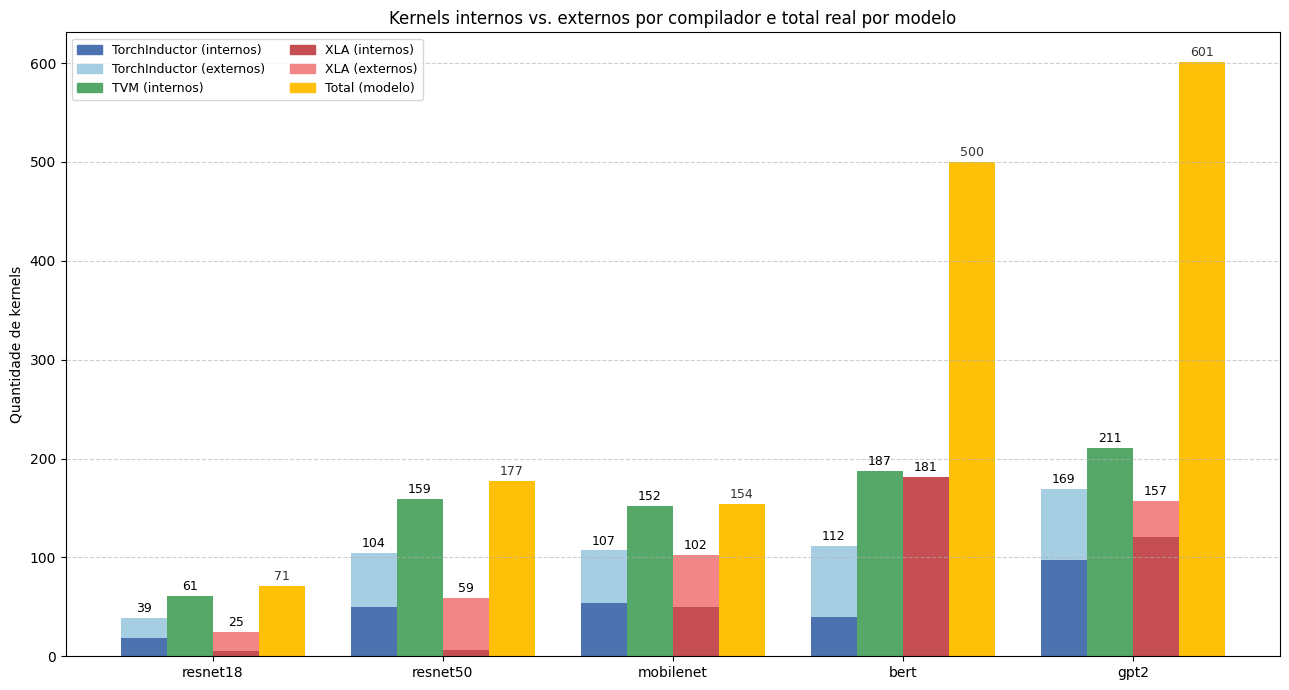
\includegraphics[width=1\linewidth]{images/comparacao_v2.png}
    \caption{Taxa de fusão por modelo considerando apenas \emph{kernels} internos.}
    \label{fig:fusion_rate}
\end{figure}

Na Figura vemos a taxa de número de kernels fundidos nos três backends para os 4 modelos. Embora ambos os \textbf{TorchInductor} e \textbf{XLA} conseguem fundir mais \textit{kernels} que o \textbf{TVM}, a taxa de fusão do \textbf{XLA} é superior em todos os modelos exceto BERT (Figura ~\ref{fig:fusion_rate}). A dominância de \textbf{TorchInductor} e \textbf{XLA} é mais clara na Figura~\ref{fig:kernels_interno}. Nela, notamos um peso maior das dependências externas, (\textit{kernels} externos), o que também impacta em tempo de fusão de operadores. Na Figura~\ref{fig:kernels_interno} também notamos a quantidade de \textit{kernels} internos por backend em cada modelo. 

\begin{figure}[h]
    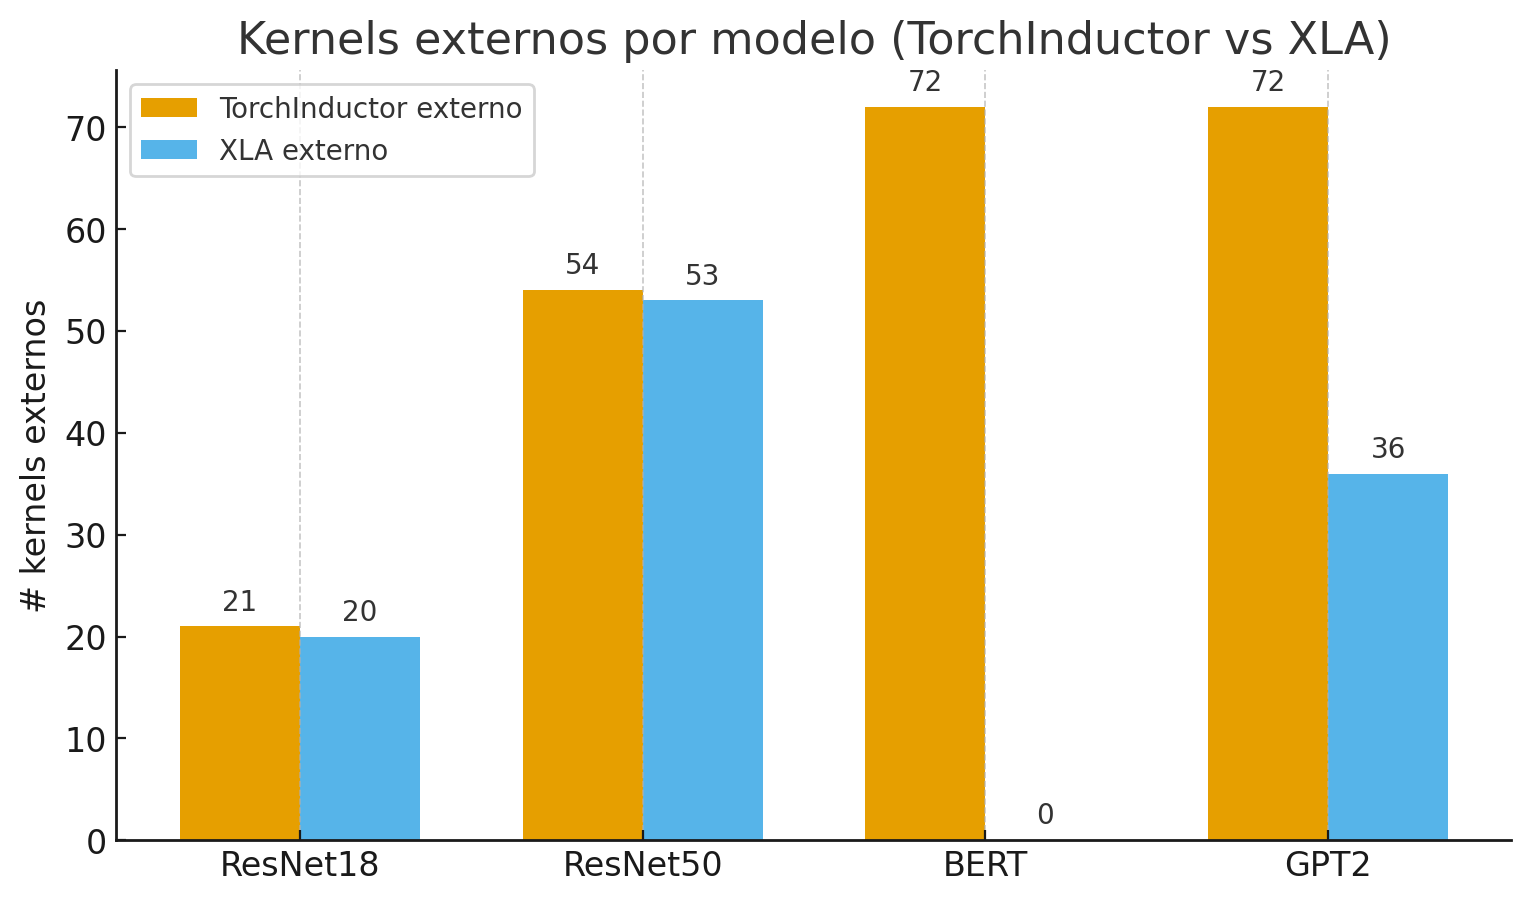
\includegraphics[width=\linewidth]{images/kernels_externo.png}
    \caption{Número de \textit{kernels} externos.}
    \label{fig:kernels_externo}
\end{figure}

\begin{figure}[h]
    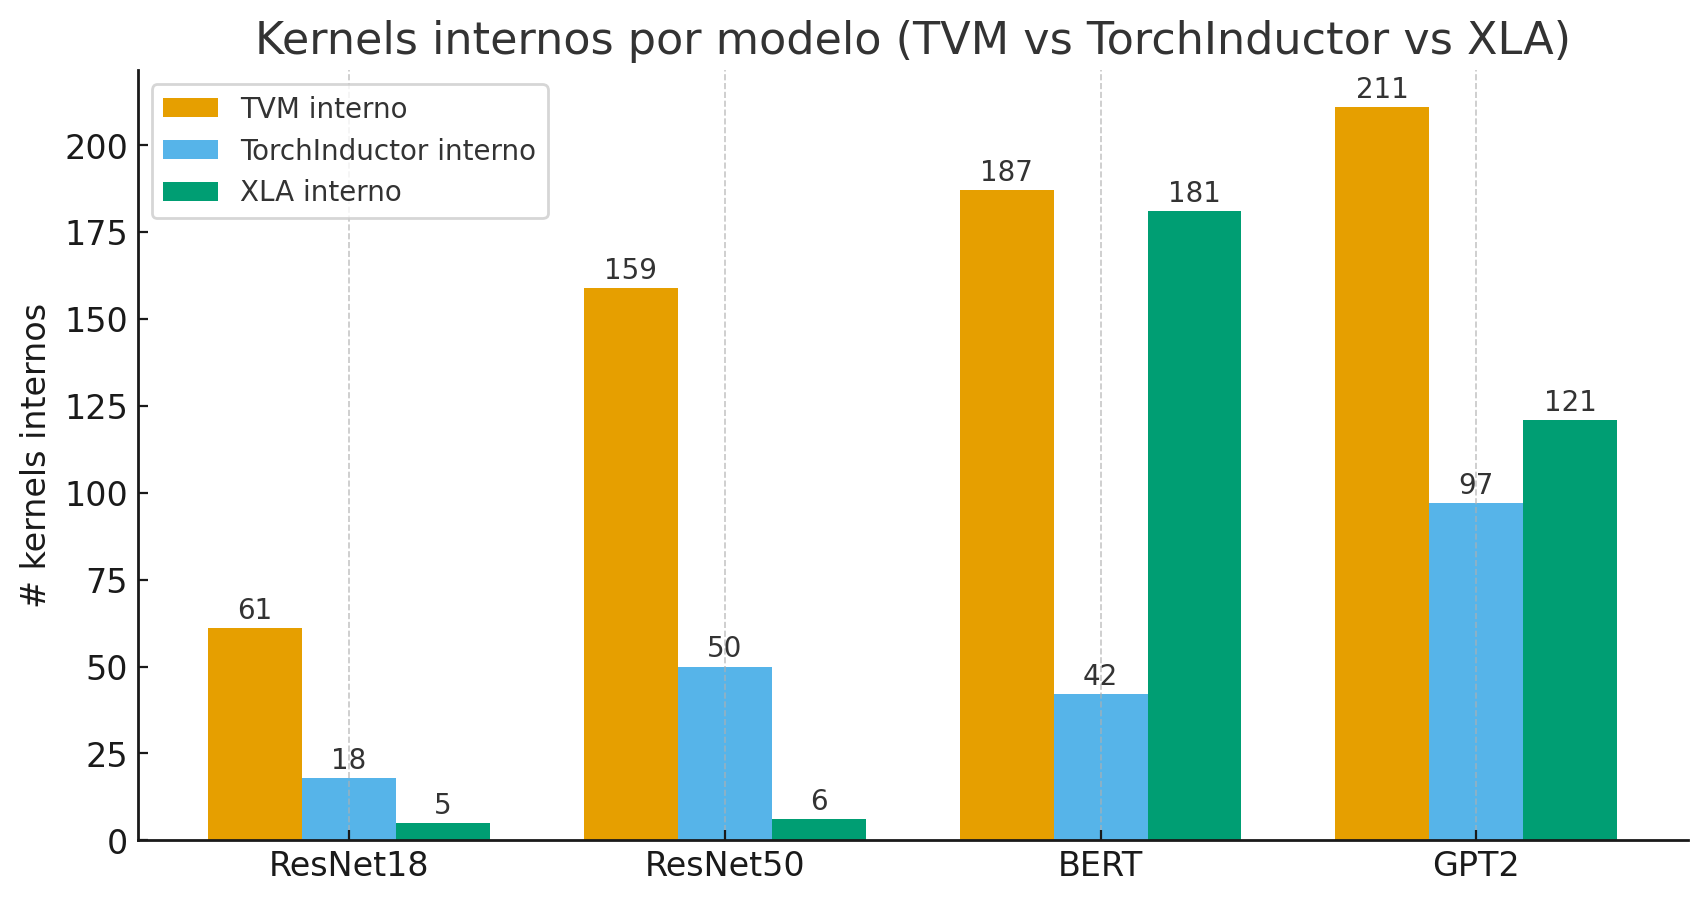
\includegraphics[width=\linewidth]{images/kernels_interno.png}
    \caption{Número de \textit{kernels} internos.}
    \label{fig:kernels_interno}
\end{figure}

% \begin{figure}[h]
%     \centering
%     % First image
%     \subfloat[\label{fig:kernels_externo}Número de \emph{kernels externos} no TorchInductor e XLA por modelo.]{%
%        
\includegraphics[width=0.45\linewidth]{kernels_externo.png}}
%     \hfill
%     % Second image
%     \subfloat[\label{fig:kernels_interno}Número de \emph{kernels internos} nos três compiladores por modelo.]{%
%        
\includegraphics[width=0.45\linewidth]{kernels_interno.png}}
% \end{figure}


% % --- Figura 2: Kernels externos ---
% \begin{figure}[h]
%     \centering
%     
\includegraphics[width=0.7\linewidth]{kernels_externo.png}
%     \caption{Número de \emph{kernels externos} no TorchInductor e XLA por modelo.}
%     \label{fig:kernels_externo}
% \end{figure}

% % --- Figura 3: Kernels internos ---
% \begin{figure}[h]
%     \centering
%     
\includegraphics[width=0.7\linewidth]{kernels_interno.png}
%     \caption{Número de \emph{kernels internos} nos três compiladores por modelo.}
%     \label{fig:kernels_interno}
% \end{figure}

% , \ref{fig:kernels_externo} e \ref{fig:kernels_interno} 

% \begin{itemize}
%     \item como cada compilador decompõe o modelo em \emph{kernels internos} (Fig.~\ref{fig:kernels_interno}).
% \end{itemize}

% grafico de linha por modelo. fusao nos kernels internos: torchinductor interno, xla interno, xla externo, tvm interno. em porcentagem 

% grafico: xla VS torchinductor - kernels externos. com #  de kernels externos por compilador e em cada modelo
% pra cada modelo, 2 barras: torch externo, xla externo

% apaga o proximo e substitui pelos  2

\subsection{Redes Residuais}

\begin{table*}[h]
\centering
\caption{ResNet-18 — tempos de \textbf{compilação}/\textbf{execução} (ms). Valores: média $\pm$ dp [IC95\%]; $n=50$, 10 aquecimentos.}
\label{tab:resnet18_compile_exec}
\small

\adjustbox{max width=\textwidth}{%
\begin{tabular}{llcc}
\toprule
\textbf{Framework} & \textbf{Entrada (N,C,H,W)} & \textbf{Compilação} & \textbf{Execução} \\
\midrule
\multirow{5}{*}{TorchInductor}
& (1,\,3,\,224,\,224)   & \worst{8550}  & \best{1.76 $\pm$ 0.03 [1.75, 1.77]} \\
& (16,\,3,\,224,\,224)  & \worst{6233}  & \worst{11.78 $\pm$ 0.18 [11.71, 11.85]} \\
& (64,\,3,\,224,\,224)  & \worst{6348}  & \worst{40.51 $\pm$ 0.42 [40.36, 40.66]} \\
& (1,\,3,\,512,\,512)   & \worst{6168}  & \worst{4.70 $\pm$ 0.05 [4.68, 4.72]} \\
& (1,\,3,\,1024,\,1024) & \worst{5929}  & \worst{15.07 $\pm$ 0.16 [15.01, 15.13]} \\
\midrule
\multirow{5}{*}{TVM}
& (1,\,3,\,224,\,224)   & \worst{10273} & \worst{6.94 $\pm$ 0.07 [6.91, 6.97]} \\
& (16,\,3,\,224,\,224)  & \worst{10004} & \worst{82.53 $\pm$ 0.62 [82.30, 82.76]} \\
& (64,\,3,\,224,\,224)  & \worst{9899}  & \worst{321.09 $\pm$ 1.90 [320.39, 321.79]} \\
& (1,\,3,\,512,\,512)   & \worst{4992}  & \worst{27.00 $\pm$ 0.31 [26.89, 27.11]} \\
& (1,\,3,\,1024,\,1024) & \worst{9256}  & \worst{103.97 $\pm$ 0.84 [103.65, 104.29]} \\
\midrule
\multirow{5}{*}{XLA}
& (1,\,3,\,224,\,224)   & \best{2457}  & \worst{1.99 $\pm$ 0.03 [1.98, 2.00]} \\
& (16,\,3,\,224,\,224)  & \best{2917}  & \best{11.39 $\pm$ 0.15 [11.33, 11.45]} \\
& (64,\,3,\,224,\,224)  & \best{4640}  & \best{38.79 $\pm$ 0.39 [38.64, 38.94]} \\
& (1,\,3,\,512,\,512)   & \best{3050}  & \best{4.17 $\pm$ 0.05 [4.15, 4.19]} \\
& (1,\,3,\,1024,\,1024) & \best{3297}  & \best{12.75 $\pm$ 0.12 [12.71, 12.79]} \\
\bottomrule
\end{tabular}
}
\end{table*}

\begin{table*}[h]
\centering
\caption{ResNet-50 — tempos de \textbf{compilação}/\textbf{execução} (ms). Valores: média $\pm$ dp [IC95\%]; $n=50$, 10 aquecimentos.}
\label{tab:resnet50_compile_exec}
\small

\adjustbox{max width=\textwidth}{%
\begin{tabular}{llcc}
\toprule
\textbf{Framework} & \textbf{Entrada (N,C,H,W)} & \textbf{Compilação} & \textbf{Execução} \\
\midrule
\multirow{5}{*}{TorchInductor}
& (1,\,3,\,224,\,224)   & \worst{13902} & \best{3.55 $\pm$ 0.04 [3.54, 3.56]} \\
& (16,\,3,\,224,\,224)  & \worst{13125} & \best{29.20 $\pm$ 0.35 [29.10, 29.30]} \\
& (64,\,3,\,224,\,224)  & \worst{11952} & \worst{107.14 $\pm$ 1.29 [106.77, 107.51]} \\
& (1,\,3,\,512,\,512)   & \worst{12373} & \worst{10.73 $\pm$ 0.13 [10.69, 10.77]} \\
& (1,\,3,\,1024,\,1024) & \worst{11767} & \worst{37.16 $\pm$ 0.45 [37.03, 37.29]} \\
\midrule
\multirow{5}{*}{TVM}
& (1,\,3,\,224,\,224)   & \worst{10273} & \worst{19.47 $\pm$ 0.18 [19.42, 19.52]} \\
& (16,\,3,\,224,\,224)  & \worst{10004} & \worst{247.63 $\pm$ 2.23 [247.00, 248.26]} \\
& (64,\,3,\,224,\,224)  & \worst{9896}  & \worst{986.00 $\pm$ 8.87 [983.48, 988.52]} \\
& (1,\,3,\,512,\,512)   & \worst{9648}  & \worst{91.01 $\pm$ 0.82 [90.78, 91.24]} \\
& (1,\,3,\,1024,\,1024) & \worst{9256}  & \worst{347.04 $\pm$ 3.12 [346.15, 347.93]} \\
\midrule
\multirow{5}{*}{XLA}
& (1,\,3,\,224,\,224)   & \best{4748}  & \worst{4.21 $\pm$ 0.04 [4.20, 4.22]} \\
& (16,\,3,\,224,\,224)  & \best{5936}  & \worst{29.71 $\pm$ 0.30 [29.62, 29.80]} \\
& (64,\,3,\,224,\,224)  & \best{9581}  & \best{101.00 $\pm$ 1.01 [100.71, 101.29]} \\
& (1,\,3,\,512,\,512)   & \best{4671}  & \best{10.70 $\pm$ 0.11 [10.67, 10.73]} \\
& (1,\,3,\,1024,\,1024) & \best{6028}  & \best{33.77 $\pm$ 0.34 [33.67, 33.87]} \\
\bottomrule
\end{tabular}
}
\end{table*}

Nas arquiteturas \textbf{ResNet-18} e \textbf{ResNet-50}, os três backends revelam diferenças estruturais na forma como cada sistema lida com fusões, granularidade e delegação de operações a bibliotecas externas.

O \textbf{TVM}, apresenta o maior número de \emph{kernels} devido à sua forma de representação: as operações de \textit{convolução} e \textit{batch normalization} chegam marcadas como \emph{opacas}, e o compilador não tem visibilidade para aplicar fusões agressivas. Mesmo a \textit{ReLU} permanece isolada. O resultado é um pipeline fragmentado, com fusões simples e pouca redução estrutural do grafo.

O \textbf{TorchInductor} depende amplamente do \textbf{cuDNN} para convoluções, o que o impede de fundir convolução, \textit{BatchNorm} e ativação em um único \textit{kernel}. Porém, ele faz fusões \textit{BatchNorm+ReLU} dentro de \emph{kernels} Triton. Há menos disparos e os grafos são mais compactos que os do TVM. Entretanto, o uso de Triton para operações elementares e reduções aumenta o tempo de geração de código, \textbf{que cresce proporcionalmente com o modelo} (Tabelas~\ref{tab:resnet18_compile_exec} ,~\ref{tab:resnet50_compile_exec}).

Isso reduz o número total de lançamentos e, em geral, resulta em grafos mais compactos que os do TVM. Contudo, essa abordagem híbrida traz um custo: o uso de Triton para inúmeras operações \textit{elementwise} e reduções aumenta o tempo de \textit{codegen} e faz com que o tempo de compilação cresça proporcionalmente ao tamanho do modelo, especialmente perceptível ao passar da ResNet-18 para a ResNet-50.

% O XLA, porém, adota uma estratégia agressiva ao combinar \textit{convolução + bias + batch norm + ativação} em uma única chamada ao cuDNN [X:falta citacao. doc?]. Isso reduz o número de \emph{kernels} finais e produz pipelines mais coesos. O impacto é visível na redução do tempo de compilação em relação aos outros backends.

No XLA, a partir da análise dos HLOs, observamos que o compilador realiza fusões agressivas combinando \emph{convolution + bias + batch norm + activation} em uma única chamada ao cuDNN. Essa fusão reduz o número de \emph{kernels} finais e resulta em pipelines mais coesos. Experimentalmente, esse comportamento mostrou impacto direto na redução do tempo de compilação quando comparado a outros backends.

% [X: isso abaixo é para vc explicar na apresentacao]
% Em síntese, o TVM prioriza clareza estrutural, o TorchInductor equilibra flexibilidade com desempenho, e o XLA puxa para fusões maximalistas e forte integração com bibliotecas nativas, o que explica sua vantagem consistente na execução.

\subsection{Arquiteturas baseadas em atenção (BERT)}

\begin{table*}[h]
\centering
\caption{BERT — tempo de \textbf{compilação}/\textbf{execução} (ms) por framework e configuração de entrada (\textit{batch, seq\_len}). Execução: média $\pm$ dp [IC95\%]; $n=50$, 10 aquecimentos.}
\label{tab:bert_compile_exec}
\small

\adjustbox{max width=\textwidth}{%
\begin{tabular}{llcc}
\toprule
\textbf{Framework} & \textbf{Entrada (batch, seq\_len)} & \textbf{Compilação} & \textbf{Execução} \\
\midrule
\multirow{3}{*}{TorchInductor}
& (1,\,64)   & \worst{13449} & \best{3.49 $\pm$ 0.63 [3.31, 3.67]} \\
& (1,\,128)  & \worst{12071} & \best{5.11 $\pm$ 0.73 [4.90, 5.32]} \\
& (8,\,128)  & \worst{11396} & \worst{31.51 $\pm$ 0.95 [31.24, 31.78]} \\
\midrule
\multirow{3}{*}{TVM}
& (1,\,64)   & \best{2492}  & \worst{6.78 $\pm$ 0.34 [6.66, 6.90]} \\
& (1,\,128)  & \best{1564}  & \worst{9.85 $\pm$ 0.49 [9.67, 10.03]} \\
& (8,\,128)  & \best{1464}  & \worst{63.00 $\pm$ 1.26 [62.55, 63.45]} \\
\midrule
\multirow{3}{*}{XLA}
& (1,\,64)   & \worst{5474}  & \worst{3.88 $\pm$ 0.26 [3.81, 3.95]} \\
& (1,\,128)  & \worst{5074}  & \worst{5.27 $\pm$ 0.25 [5.20, 5.34]} \\
& (8,\,128)  & \worst{5317}  & \best{29.95 $\pm$ 0.32 [29.86, 30.04]} \\
\bottomrule
\end{tabular}
}
\end{table*}

O modelo \textbf{BERT}, possui um padrão de fusões distinto que reflete a arquitetura centrada em \textit{matmuls}~\cite{pati2021demystifying}, projeções QKV e operações de normalização e ativação.

O \textbf{TVM} tende a produzir \emph{kernels} menores e mais numerosos. Isso leva a fragmentação do grafo, semelhante ao visto nas ResNets, mas no BERT, sua taxa de fusão é maior graças à estrutura, que possui longas cadeias elementares facilmente colapsáveis.

O \textbf{TorchInductor} explora fusões em torno de minimizar o acesso à memória. Ele delega os \textit{matmuls} para bibliotecas externas (por exemplo, cuBLAS) \cite{pytorch2022} e concentra-se nos \emph{kernels} Triton. A partir da análise direta dos artefatos e kernels gerados pelo TorchInductor, observou-se que o compilador sintetiza estruturas que correspondem, na prática, a blocos típicos de \emph{Transformers}. Esses templates de kernels são reutilizados ao longo da rede, o que leva à redução no número de lançamentos, embora à custa de maior tempo de compilação.

% como \tcode{embedding} + somas residuais + \tcode{LayerNorm}, \tcode{GELU} completo e \tcode{softmax} de atenção com máscara e escala [X: referencie o paper do pytorch2]. Os \emph{templates} Triton são reutilizados ao longo da rede, resultando em um número total de \emph{kernels} lançados menor que o dos demais sistemas, às custas de maior tempo de compilação.

O \textbf{XLA}, termina com mais \emph{kernels} que o TorchInductor, mas praticamente todas são \textbf{fusões HLO}: desde fusões de \textit{GEMM} (\tcode{gemm\_fusion\_dot}, com pesos QKV concatenados e epílogos incorporados) até fusões dedicadas ao \tcode{softmax} de atenção (\tcode{triton\_softmax\_computation}), e grandes fusões do tipo \tcode{kLoop}/\tcode{kInput} que implementam \tcode{LayerNorm} e \tcode{GELU} completos. Essas fusões de \textit{GEMM} correspondem \textbf{às mesmas 72 multiplicações de matrizes observadas no TorchInductor}; contudo, por serem fusões internas altamente especializadas, elas já incorporam operações de \textit{bias}, concatenação QKV e ajustes de \textit{layout} dentro de um único \emph{kernel}. Quando o \emph{batch} aumenta, o custo dessas \textit{GEMMs} \textbf{passa a dominar o tempo total de execução}, o que torna o overhead devido ao maior número de \textit{kernels} irrelevante. Esse comportamento é especialmente visualizazado no cenário \((8, 128)\) (Tabela~\ref{tab:bert_compile_exec}).

Em suma, o modelo BERT evidencia como as diferenças arquiteturais impactam na estratégia de cada compilador.

% como diferenças arquiteturais modulam a estratégia de fusão de cada compilador: enquanto nas ResNets o XLA se mostra mais agressivo em reduzir o número de \emph{kernels}, no BERT o TorchInductor lança menos \emph{kernels} e explora fusões altamente especializadas para \emph{Transformers}, ao passo que o XLA mantém melhor tempo de compilação e se mantém competitivo em execução — superando o Inductor em lotes maiores, ainda que perca levemente em lotes pequenos, justamente porque, nessa configuração, as \textit{GEMMs} especializadas passam a dominar o custo total.

\subsection{Modelos baseados em atenção autoregressiva (GPT-2)}

\begin{table*}[h]
\centering
\caption{GPT-2 — tempo de \textbf{compilação}/\textbf{execução} (ms) por framework e configuração de entrada (\textit{batch, seq\_len}). Execução: média $\pm$ dp [IC95\%]; $n=50$, 10 aquecimentos.}
\label{tab:gpt2_compile_exec}
\small

\adjustbox{max width=\textwidth}{%
\begin{tabular}{llcc}
\toprule
\textbf{Framework} & \textbf{Entrada (batch, seq\_len)} & \textbf{Compilação} & \textbf{Execução} \\
\midrule
\multirow{4}{*}{TorchInductor}
& (1,\,16)   & \worst{15003} & \worst{3.09 $\pm$ 0.33 [3.00, 3.18]} \\
& (1,\,128)  & \worst{13327} & \worst{6.12 $\pm$ 0.60 [5.95, 6.29]} \\
& (8,\,128)  & \worst{19121} & \best{30.40 $\pm$ 0.75 [30.19, 30.61]} \\
& (8,\,256)  & \worst{18353} & \worst{58.56 $\pm$ 0.74 [58.35, 58.77]} \\
\midrule
\multirow{4}{*}{TVM}
& (1,\,16)   & \worst{8253}  & \worst{7.80 $\pm$ 0.39 [7.66, 7.94]} \\
& (1,\,128)  & \worst{10312} & \worst{10.55 $\pm$ 0.53 [10.36, 10.74]} \\
& (8,\,128)  & \worst{9776}  & \worst{41.21 $\pm$ 1.24 [40.77, 41.65]} \\
& (8,\,256)  & \worst{9549}  & \worst{79.11 $\pm$ 1.98 [78.40, 79.82]} \\
\midrule
\multirow{4}{*}{XLA}
& (1,\,16)   & \best{2797}  & \best{2.81 $\pm$ 0.17 [2.76, 2.86]} \\
& (1,\,128)  & \best{3892}  & \best{5.11 $\pm$ 0.28 [5.03, 5.19]} \\
& (8,\,128)  & \best{5784}  & \worst{30.84 $\pm$ 0.72 [30.64, 31.04]} \\
& (8,\,256)  & \best{5562}  & \best{58.38 $\pm$ 0.54 [58.23, 58.53]} \\
\bottomrule
\end{tabular}
}
\end{table*}

Os blocos do GPT-2 seguem um padrão decoder-only relativamente linear — atenção auto-regressiva e MLP, cada um precedido por LayerNorm e seguido de ativação GELU, repetidos em todas as camadas. \cite{radford2019language}

O \textbf{TVM} não consegue incorporar epílogos longos, como \textit{softmax} ou \textit{LayerNorm}, em \emph{kernels} maiores, pois muitos são marcados como opacos na IR. Mesmo assim, o TVM funde epílogos curtos, como adição de \textit{bias} e, em alguns casos, \textit{GELU} além de consolidar cadeias elementares e normalizações próximas.

O \textbf{TorchInductor} adota a mesma estratégia: delega os \textit{kernels} às bibliotecas externas, e sintetiza \emph{kernels} Triton combinando normalização, ativações e \textit{softmax}. O Inductor tem um padrão de “epílogo expandido” que reduz o número de \emph{kernels}, com fusões envolvendo \textbf{LayerNorm}, \textbf{GELU} e \textbf{softmax}. Assim como no BERT, porém, essa estratégia implica maior custo de compilação, dado o tamanho e a complexidade dos \emph{kernels} Triton.

O \textbf{XLA} apresenta uma estratégia equilibrada entre granularidade e integração com bibliotecas externas. O XLA tem a capacidade de consolidar múltiplas operações auxiliares ao redor dos \textit{matmuls}, resultando em \textit{kernels} maiores, o que o leva a obter \textbf{tempos de execução mais rápidos na maioria das configurações} (tabela ~\ref{tab:gpt2_compile_exec}).

% Embora gere \emph{custom-calls} ao \tcode{cublas\$gemm}, ele envolve esses GEMMs em \textbf{fusões internas HLO} que cobrem cadeias consideravelmente amplas, incluindo \textit{bias}, \textit{reshape}, \textit{transpose}, normalização, \textit{GELU} e \textit{softmax}. Essa capacidade de consolidar múltiplas operações auxiliares ao redor dos \textit{matmuls} resulta em regiões maiores de computação por \emph{kernel}, preservando ao mesmo tempo compatibilidade com kernels altamente otimizados do cuBLAS. Na prática, isso leva o XLA a obter \textbf{tempos de execução mais rápidos na maioria das configurações}.

Embora as taxas de fusão finais entre \textbf{TorchInductor} e \textbf{XLA} sejam próximas, o padrão de fusão mais estruturado do XLA permite que ele mantenha desempenho superior em tempo de execução no GPT-2.

% Em termos de tempo de execução, o \textbf{XLA} foi melhor em \textbf{todos} os modelos, evidenciando que embora o número de \textit{kernels} seja maior, a qualidade de fusões e epílogos pode superar a sobrecarga devido a quantidade de disparos.

Em termos de tempo de execução, o \textbf{XLA} foi melhor em \textbf{todos} os modelos, evidenciando que tanto granularidade quanto qualidade das fusões são métricas relevantes e devem ser analisadas juntas.

% [X: Quando perguntarem - porque? Aí vc coloca na apresentacao o que esta abaixo. explicando o prq XLA é mais rapido. mas nao precisa explicar detalhadamente aqui. coloque uma referencia]
% \subsection{Síntese dos resultados de tempo}

% O compilador XLA foi mais rápido em \textbf{todos} os modelos.

% Em suma: (i) nas CNNs, os epílogos do cuDNN (conv+bias+ativação) e a supressão de \emph{kernels} intermediários explicam os \textbf{grandes ganhos} nas ResNets; (ii) no GPT-2, as fusões internas ao redor da atenção também trazem \textbf{melhorias substanciais}; e (iii) mesmo em BERT — onde o XLA gerou \emph{mais} \emph{kernels} — o tempo final foi \textbf{menor}, evidenciando que a \textbf{qualidade das fusões e epílogos} pode superar a simples contagem de \emph{kernels}.

% O \textbf{PyTorch} adota um pipeline distinto e, do ponto de vista do \textbf{tempo de compilação}, menos eficiente que o XLA: envolve \emph{FX tracing}, decomposições e \emph{codegen} de múltiplos \emph{kernels} Triton orquestrados a partir de Python; já o \textbf{XLA} aplica reescritas determinísticas no HLO em um pipeline monolítico em C++, explorando \textbf{fusões de biblioteca} (p.ex., cuDNN/cuBLASLt) com baixo \emph{overhead}. \textit{Como comentado ao longo da Seção de Resultados}, os tempos coletados evidenciam uma discrepância marcante (sobretudo em \emph{compilação}) entre XLA e TorchInductor e, em conjunto com a análise de artefatos e da contagem/granularidade de \emph{kernels}, motivaram a hipótese de que o \emph{codegen} do TorchInductor estaria degradando o tempo de compilação além do esperado pela própria arquitetura do sistema. Para averiguar essa hipótese, introduzimos a subseção \textbf{Folds}: criamos um \textbf{passe no \textit{FX} graph} das ResNets (ResNet-18/50) que realiza o \textbf{fold Conv+BN} (absorvendo a \tcode{BatchNorm} nos parâmetros da \tcode{Conv}) por \textit{pattern matching} leve. Em teoria, isso elimina a necessidade do \emph{codegen} Triton para o \emph{kernel} fundido \tcode{BatchNorm+ReLU} no TorchInductor, reduzindo o \textbf{tempo de compilação} com impacto mínimo no \textbf{tempo de execução}.



\subsection{Fold}

\begin{table}[h]
\centering
\caption{ResNet-18 (TorchInductor) — efeito do \textit{fold} de BN em Conv: tempos de compilação/execução (ms).}
\label{tab:resnet18_fold_bn}
\small
\adjustbox{max width=\linewidth}{%
\begin{tabular}{lrrrrrr}
\toprule
\textbf{Entrada} & \textbf{Comp. s/ fold} & \textbf{Comp. c/ fold} & \(\Delta\)\textbf{ Comp.} & \textbf{Exec. s/ fold} & \textbf{Exec. c/ fold} & \(\Delta\)\textbf{ Exec.} \\
\midrule
(1,3,224,224)   & 8550  & 4305.06 & \(-49.6\%\) & 1.76  & 1.97  & \(+12.0\%\) \\
(16,3,224,224)  & 6233  & 2566.06 & \(-58.9\%\) & 11.78 & 11.70 & \(-0.7\%\)  \\
(64,3,224,224)  & 6348  & 2790.42 & \(-56.0\%\) & 40.51 & 42.69 & \(+5.4\%\)  \\
(1,3,512,512)   & 6168  & 2909.80 & \(-52.9\%\) & 4.70  & 4.80  & \(+2.2\%\)  \\
(1,3,1024,1024) & 5929  & 2582.70 & \(-56.5\%\) & 15.07 & 15.05 & \(-0.1\%\)  \\
\bottomrule
\end{tabular}
}
\end{table}


\begin{table}[h]
\centering
\caption{ResNet-50 (TorchInductor) — efeito do \textit{fold} de BN em Conv: tempos de compilação/execução (ms).}
\label{tab:resnet50_fold_bn}
\small

\adjustbox{max width=\linewidth}{%
\begin{tabular}{lrrrrrr}
\toprule
\textbf{Entrada} & \textbf{Comp. s/ fold} & \textbf{Comp. c/ fold} & \(\Delta\)\textbf{ Comp.} & \textbf{Exec. s/ fold} & \textbf{Exec. c/ fold} & \(\Delta\)\textbf{ Exec.} \\
\midrule
(1,3,224,224)   & 13902 & 11467.60 & \(-17.5\%\) & 3.55   & 3.48   & \(-2.0\%\) \\
(16,3,224,224)  & 13125 & 7401.21  & \(-43.6\%\) & 29.20  & 28.832 & \(-1.3\%\) \\
(64,3,224,224)  & 11952 & 8576.11  & \(-28.3\%\) & 107.14 & 105.917& \(-1.1\%\) \\
(1,3,512,512)   & 12373 & 7753.59  & \(-37.3\%\) & 10.73  & 10.601 & \(-1.2\%\) \\
(1,3,1024,1024) & 11767 & 7618.43  & \(-35.3\%\) & 37.16  & 37.088 & \(-0.2\%\) \\
\bottomrule
\end{tabular}
}
\end{table}

\paragraph{Fold (ResNets).}
A aplicação do \textit{fold} antes do passe de fusão reduz o tempo de compilação nas duas ResNets (Tabelas~\ref{tab:resnet18_fold_bn} e \ref{tab:resnet50_fold_bn}). O impacto varia com o tamanho do modelo. O \textit{fold} de \textbf{BatchNorm} atua como uma otimização estrutural simples no interior dos \emph{kernels}, facilitando a escrita da fusão deles. Porém, altera de forma significativa o desempenho em tempo de execução como na primeira linha da tabela \ref{tab:resnet18_fold_bn} (+12\% em ResNet-18).

\begin{table}[h]
\centering
\caption{BERT (TorchInductor) — efeito do \textit{fold} da parte afim da LayerNorm em Linear: tempos de compilação/execução (ms).}
\label{tab:bert_ln_fold}
\small

\adjustbox{max width=\linewidth}{%
\begin{tabular}{lrrrrrr}
\toprule
\textbf{Entrada} & \textbf{Comp. s/ fold} & \textbf{Comp. c/ fold} & \(\Delta\)\textbf{ Comp.} & \textbf{Exec. s/ fold} & \textbf{Exec. c/ fold} & \(\Delta\)\textbf{ Exec.} \\
\midrule
(1,64)   & 13449 & 6345.70 & \(-52.8\%\) & 3.49 & 3.22  & \(-7.7\%\) \\
(1,128)  & 12071 & 6106.58 & \(-49.4\%\) & 5.11 & 5.25  & \(+2.8\%\) \\
(8,128)  & 11396 & 6119.32 & \(-46.3\%\) & 31.51& 30.28 & \(-3.9\%\) \\
\bottomrule
\end{tabular}
}
\end{table}

\paragraph{Fold (BERT).}
No BERT, a \textbf{LayerNorm} (LN) em inferência divide-se em duas partes: (i) a \emph{normalização} e (ii) a \emph{parte afim} (\(\gamma,\beta\)) (ver Apêndice~A). No \textbf{TorchInductor}, quando LN e sua parte afim aparecem compostas no grafo, o compilador gera um único \emph{kernel} Triton que inclui normalização, operações element-wise (\tcode{mul}/\tcode{add}) e múltiplos \emph{loads} adicionais. Essa combinação torna o \emph{kernel} mais denso e eleva o custo de \emph{codegen}.

Ao aplicar o \textbf{fold} — absorvendo \(\gamma\) e \(\beta\) na \tcode{Linear} subsequente (escalando colunas de \(W\) e ajustando o viés) — a LN torna-se apenas uma normalização \emph{sem affine}. Isso remove do \emph{kernel} Triton as operações extras e reduz significativamente sua densidade, simplificando o trabalho do gerador de código e, assim, \textbf{diminuindo o tempo de compilação}, ainda que o número de \emph{kernels} permaneça o mesmo.

O \emph{fold} também reduz a lacuna em relação ao \textbf{XLA}. No \textbf{XLA}, a LN aparece dentro de regiões de fusão maiores, compiladas de forma monolítica, sem a orquestração Python/Triton e sem materializar a etapa afim como operação isolada. 

% [X: abaixo só pode ter se tiver referencia]
% Na análise de artefatos, os kernels de \emph{residual+LN} no Inductor carregam explicitamente \(\gamma,\beta\) como parâmetros e emitem instruções adicionais de \tcode{mul}/\tcode{add} e \emph{loads} desses tensores, o que aumenta o custo de geração de código. Ao remover \(\gamma,\beta\) dos kernels de LN e empurrar essa parte afim para os pesos/viés da \tcode{Linear} subsequente, cortamos trabalho de compilação justamente onde ele é mais repetido (várias LNs por bloco/camada), estreitando a diferença de \emph{compile-time} em relação ao XLA. Empiricamente, observamos reduções substanciais no tempo de compilação ao aplicar esse \emph{fold}, com latências de execução mantendo-se estáveis ou variando apenas levemente.

Em síntese: O \textbf{TVM} apresenta maior granularidade (mais \emph{kernels}) e fusões mais conservadoras; o \textbf{TorchInductor} combina \emph{kernels} via Triton com chamadas a bibliotecas externas; o \textbf{XLA} realiza fusões mais agressivas em Transformers, mas mantém chamadas personalizadas.

O \textbf{TorchInductor} tende a gerar \emph{kernels} separados para a convolução (delegada a bibliotecas) e para operações subsequentes compiladas via Triton; já o \textbf{XLA} costuma fundir essas operações em um único grafo e delegar a execução, reduzindo geração de código e disparos.

Os testes com o \textit{fold} antes da conversão do grafo \textbf{mostram melhora relevante no tempo de compilação} do PyTorch. Isso indica uma ordem de otimizações ineficiente no backend do PyTorch. Nosso trabalho defende que a operação \textit{fold} deve ser realizada antes da fusão de operadores, pois ela simplifica o grafo antes do \emph{codegen}. A Figura ~\ref{fig:foldeq} suporta nossa alegação.

% Algebra + grafico da variação
Ganhos em tempo de execução não são determinísticos em nenhum dos três modelos (ResNets e BERT), pela natureza de otimização de código. A análise evidencia que \textbf{tempo de compilação maior não implica, por si, em fusões melhores}. Na ResNet-50, observamos melhoria no tempo de execução após o \textbf{\textit{fold}} em todos os casos de teste. Enxergamos então a necessidade da construção de um benchmark e modelo algébrico para decidir qual backend de ML utilizar em termos da relação tempo de compilação e tempo de execução. Na Figura~\ref{fig:foldeq}, por exemplo, calculamos o número de equivalência $n_{eq}$ (definido na Seção 4.3) para a fusão \textit{fold}. Números negativos foram simplificados para zero por significarem que 0 \textit{batches} são necessários para obter-se tempo ganho em tempo de execução.

% --- Figura 5: Ponto de equivalencia ---
\begin{figure}[h]
    \centering
    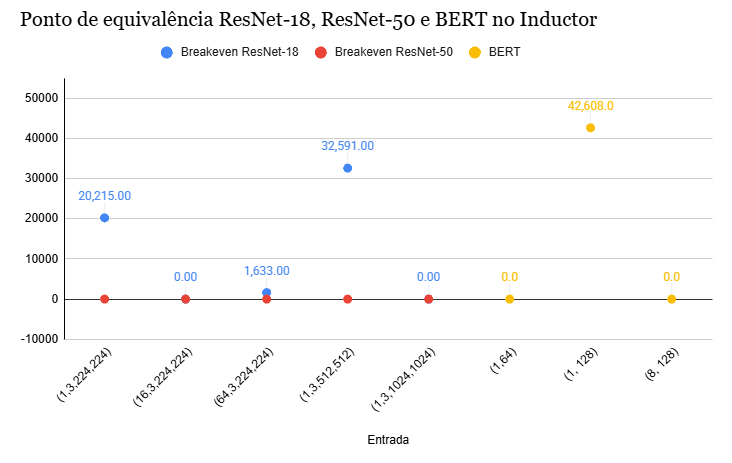
\includegraphics[width=1\linewidth]{images/equivalencia.png}
    \caption{Ponto de equivalência (número de execuções a partir do qual vale a pena compilar com o passe de fold) no backend TorchInductor.}
    \label{fig:foldeq}
\end{figure}

% [X: Leia esse paragrafo. é o resumo do trabalho]
Esse número é importante pois é o ponto de equilíbrio (\textit{break-even}) entre o custo de uma otimização e o benefício obtido na execução. Em sistemas de ML, a fusão de operadores é cara. Se o modelo for executado apenas um número limitado de vezes, esse custo pode não ser compensado pela pequena redução no tempo de execução, ou pode até elevá-lo. Porém, o significado desse limiar está na relevância para o futuro dos modelos que se auto-reprogramam. À medida que modelos ganham a capacidade de reescrever e otimizar dinamicamente seus próprios grafos de computação, eles precisarão incorporar heurísticas de custo-benefício para decidir autonomamente quando e quais otimizações aplicar. Esse número é uma métrica fundamental no pipeline de decisão, garantindo o ciclo contínuo de adaptação e otimização dos modelos de forma eficaz e sustentável.

Realizamos a análise isolada do passe de fusão, mas o benchmark proposto pode ser expandido para outros passes e também modelos.

\subsection{Benchmark Proposto}

Desenvolveu-se um \textit{benchmark} em que a pessoa usuária escolhe a \textbf{entrada do modelo} (\(N{\times}C{\times}H{\times}W\)) e o sistema executa, para cada compilador, a medição padronizada de \textbf{tempo de compilação} e \textbf{tempo de execução por inferência} com aquela entrada. Ao final, o \textit{benchmark} reporta (i) \emph{qual compilador apresenta melhor ganho} para o número de execuções de interesse e (ii) os \textbf{intervalos de execuções} em que \emph{cada} compilador se sobressai.

Para garantir justiça na comparação, \textbf{todos os compiladores foram configurados de forma equivalente}: mesma arquitetura (ResNet-18/50), mesma precisão, mesmo dispositivo, mesmo layout quando aplicável (p.ex., \emph{channels-last}/NHWC), \tcode{eval()} ativado, janelas idênticas de \emph{warmup} e número de iterações, além de parâmetros de execução congruentes (p.ex., autotuning habilitado quando disponível). O orquestrador unifica a coleta de métricas e a serialização em JSON, garantindo reprodutibilidade.

Modelamos o custo total de cada \emph{backend} \(b\) como \(T_b(n)=a_b\,n + b_b\), em que \(a_b\) é o \textbf{tempo médio por inferência} e \(b_b\) é o \textbf{tempo de compilação}. Construindo a \textbf{envoltória inferior} dessas retas, obtemos os \textbf{pontos de troca} e, consequentemente, os \textbf{intervalos de dominância} de cada compilador.

\paragraph{Relatório (JSON) e leitura rápida.}
O \textit{benchmark} gera um arquivo JSON com: \textbf{meta} (contexto do experimento), \textbf{raw} (medidas por \emph{backend}: \tcode{compile\_ms}, \tcode{exec\_ms}, \tcode{ttfb\_ms}) e \textbf{recommendation} (modelo \(T_b(n)\), pontos de troca e segmentos de dominância). O campo \tcode{best\_at\_runs\_exec} indica diretamente o melhor \emph{backend} para o \(n\) informado.

\begin{figure}[h]
    \centering
    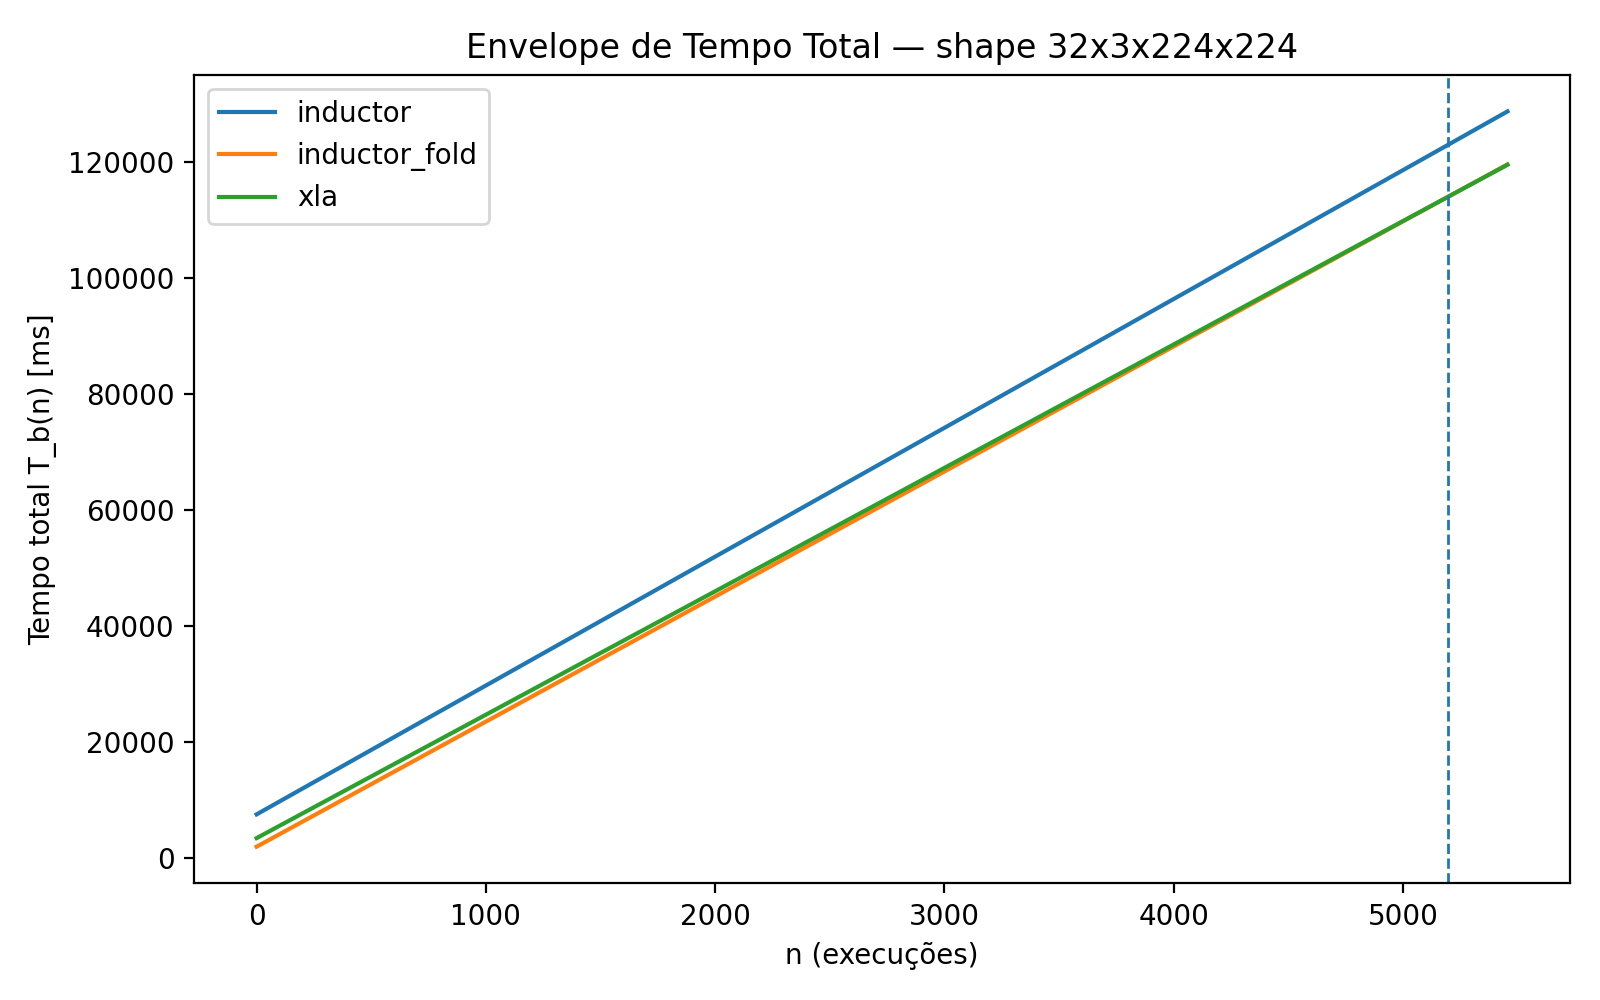
\includegraphics[width=1\linewidth]{images/envelope_exemplo.png}
    \caption{Exemplo de gráfico do \textit{benchmark}: retas \(T_b(n)=a_b n + b_b\) por \emph{backend}, com a envoltória inferior (regiões de dominância) e pontos de troca. Neste exemplo, \tcode{inductor\_fold} foi melhor até a execução 5\,197; a partir daí, XLA dominou.}
    \label{fig:envelope_exemplo}
\end{figure}

\paragraph{Como ler a Figura~\ref{fig:envelope_exemplo}.}
O eixo \(y\) inicia em \tcode{compile\_ms} (intercepto) e a inclinação é \tcode{exec\_ms}; a envoltória inferior destaca o vencedor em cada faixa de \(n\); as interseções correspondem aos pontos de troca (linhas verticais tracejadas). Se não houver interseções, o JSON vem com \tcode{breakpoints} vazio e um único \tcode{segment}.

\section{Related Work}

\textit{Performance Prediction with Machine Learning}. Research primarily focused on training regression models and neural networks to predict quantitative performance data. For instance,  ~\citet{Tousi2022} conducted a comparative analysis on the SPEC 2017 benchmark scores, evaluating models like Decision Trees, Random Forests, and Multi-Layer Perceptrons to identify the most influential hardware and software features. In a similar vein, ~\citet{Cengiz2023} demonstrated that Deep Learning models, particularly Convolutional Neural Networks (CNNs), could accurately scores from the same dataset for unseen hardware using system specifications, achieving $R^2$ scores as high as 0.98. Another significant area was cross-architecture prediction by ~\citet{Nichols2024}, who used models like XGBoost with hardware performance counters to inform multi-resource job schedulers and predict performance across different hardware platforms.

\textit{Performance Prediction with Large Language Models}. More recently, new studys using Large Language Models (LLMs) had the ideia to predict performance directly from source code arises. In their work, \citet{Wang2025Omniwise} fine-tuned a 3B-parameter LLM to predict GPU kernel performance metrics, such as memory bandwidth and cache hit rates, without requiring code execution. To our knowledge, this work is available as a preprint or published.

\section{Conclusion}

Este trabalho apresentou um protocolo unificado para avaliar compiladores de aprendizado de máquina (TorchInductor, XLA e TVM), controlando \emph{inputs}, aquecimento e número de iterações, e introduziu um critério de decisão baseado em \emph{envoltória inferior} dos tempos totais \(T_b(n)=a_b n + b_b\), onde \(a_b\) captura a latência de execução e \(b_b\) o custo de compilação. A análise comparativa mostrou que diferenças no tratamento de \emph{fusion} e de epílogos em bibliotecas como \tcode{cuDNN} explicam boa parte das variações observadas: o XLA tende a se beneficiar quando consegue delegar sequências como \tcode{Conv+BatchNorm+ReLU} a uma única \emph{custom call}, enquanto o TorchInductor, no caminho atual de \emph{inference}, paga sobrecusto de \emph{codegen} e de lançamentos adicionais ao emitir \tcode{BN+ReLU} como kernel separado (via Triton). Também observamos que a dominância de cada backend depende do regime de \(n\): em situações de poucas execuções, escolhas com compilação mais barata ganham; à medida que \(n\) domina, estratégias com maior grau de fusão de kernels prevalecem.

\paragraph{Limitações.}
Apesar do cuidado metodológico, ainda há espaço para ampliar a robustez estatística (p.\,ex., reportar intervalos de confiança para todos os cenários) e para diversificar o ambiente (outras GPUs/CPUs e versões de \tcode{driver}/\tcode{cuDNN}). Além disso, aspectos da exportação dos CFG's podem impactar a fusão de kernels não canônicos em alguns backends.

Outra limitação está na própria hipótese de linearidade do modelo \(T_b(n)=a_b n + b_b\): ao assumir que o custo por batch é aproximadamente constante e que todo o custo fixo é pago no primeiro batch, o modelo abstrai efeitos de cache, estratégias de \emph{autotuning} e eventuais recompilações disparadas por \emph{shapes} dinâmicos, que podem tornar o comportamento efetivo mais próximo de um modelo por partes do que de uma única reta. Na prática, os coeficientes \(a_b\) e \(b_b\) devem ser lidos como estatísticas-resumo da faixa de \(n\) que foi medida, e não como predições exatas para qualquer regime de uso. Trabalhos futuros podem refinar essa dimensão reportando métricas de ajuste (por exemplo, o \(R^2\) da regressão) e investigando modelos não lineares ou \emph{piecewise} em cenários com maior variabilidade temporal.

Além da comparação entre backends, este trabalho também avaliou transformações de \emph{fold} no grafo do \textbf{TorchInductor}, visando reduzir o custo de compilação sem alterar a semântica do modelo. Em arquiteturas convolucionais (ResNet-18/50), o \emph{fold} de \tcode{BatchNorm} em \tcode{Conv} reparametriza pesos e vieses da convolução e remove a \tcode{BatchNorm} explícita do grafo em modo de \emph{eval}. Isso não transforma a sequência \tcode{Conv+BatchNorm+ReLU} em um único kernel — ao contrário do XLA, que frequentemente delega toda a cadeia a uma única \emph{custom call} —, mas reduz o volume de \emph{codegen}, pois reparametrizar a \tcode{Conv} é muito mais barato do que gerar um kernel Triton separado para \tcode{BN+ReLU}.

Em modelos baseados em atenção, como o BERT, aplicamos um \emph{fold} análogo na combinação \tcode{LayerNorm+Linear}: a parte afim da \tcode{LayerNorm} ($\gamma$, $\beta$) é absorvida nos pesos e vieses da \tcode{Linear} subsequente, de modo que o TorchInductor passa a compilar apenas uma \tcode{LayerNorm} “pura”, responsável apenas pela normalização. Isso elimina a necessidade de um kernel de \tcode{LayerNorm} mais complexo (normalização + parte afim) e diminui o \emph{codegen} associado, de forma semelhante ao efeito observado com \tcode{BatchNorm}.


A extensão direta deste estudo é viabilizar a fusão de \tcode{Conv+BatchNorm+ReLU} no caminho de \emph{inference} do \textbf{TorchInductor}. A proposta consiste em (i) realizar o \emph{fold} de \tcode{BN} na \tcode{Conv} em modo \tcode{eval()} ajustando \((W', b')\); (ii) acionar o epílogo \tcode{ReLU} diretamente na \tcode{cuDNN} via \tcode{aten::cudnn\_convolution\_relu(...)} (como acontece no XLA); e (iii) integrar um \emph{pattern-rewrite} (FX/\tcode{torch.\_inductor.pattern\_matcher}) que detecte \tcode{Conv→BN→ReLU} e faça \emph{fallback} seguro quando o epílogo não estiver disponível. A avaliação dessa fusão será incorporada ao nosso \emph{benchmark} existente, adicionando o novo ponto à \emph{envoltória} \(T_b(n)\). Espera-se reduzir TTFB e latência por menor número de kernels Triton e lançamentos, ampliando os intervalos em que o TorchInductor domina — aproximando-o do perfil observado quando o XLA delega epílogos à \tcode{cuDNN}. 

\bibliographystyle{ACM-Reference-Format}
\bibliography{ref}

\end{document}